% David
\section{Gefahrengut}
\subsection{Was sind Gefahrengüter – und warum sind sie relevant?}

Gefahrengüter sind Stoffe und Gegenstände, die beim Transport eine
Gefahr für Menschen, Umwelt oder Sachwerte darstellen. Sie werden nach
internationalen Regelwerken in neun Hauptklassen und diverse Unterklassen
eingeordnet. Für jede Klasse gelten spezifische Kennzeichnungspflichten,
Verpackungsvorschriften und Dokumentationsanforderungen.

\begin{center}
  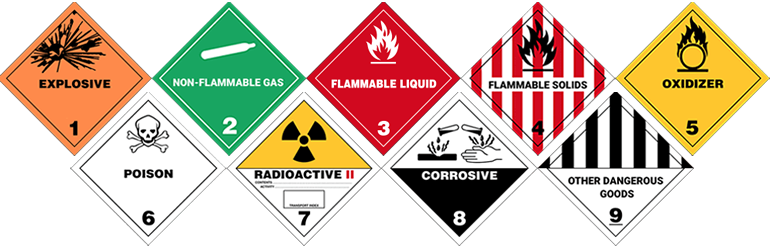
\includegraphics[width=0.7\linewidth]{./assets/gg-dangerous-shields.png}
\end{center}

Für die Beförderung existieren je nach Transportweg unterschiedliche Vorschriften:
\textbf{ADR} (Straße), \textbf{IMDG} (See), \textbf{RID} (Schiene) und \textbf{IATA} (Luft).
Diese Regelwerke definieren unter anderem zulässige Mengen, Verpackungsarten und
Begleitdokumente.

\subsection{Relevanz im ERP‐System}
\begin{itemize}
  \item Korrekte \textbf{UN-Nummer} und \textbf{Gefahrgutklasse} sind für
        Versand, Lagerung und Zollabwicklung zwingend.
  \item Fehlende oder falsche Klassifizierung führt zu
        Verzögerungen, Bußgeldern oder Transportrisiken.
  \item Automatisierte Plausibilitätsprüfungen verringern manuellen
        Aufwand und Fehlerquoten in den Stammdaten.
\end{itemize}


\section{Analyse und Verarbeitung der Gefahrgutdaten in Excel}

\subsection{Identifikation relevanter Spalten und Zeilen}
Zu Beginn der Analyse stand die manuelle Identifikation jener Spalten und Zeilen, die überhaupt mit dem 
Thema Gefahrgut in Verbindung stehen. Neben einem analytischen Vorgehen war hier auch logisches Denken gefragt: 
Es wurde schnell ersichtlich, dass die Spalte \texttt{Art\_IdentNr} ein wichtiger Indikator ist, 
da Nicht-Gefahrgüter keine UN-Deklaration und entsprechend auch keine Verpackungsvorschriften benötigen.

Im Folgenden eine Beschreibung der wichtigsten Spalten, die in diesem Zusammenhang betrachtet wurden:

\begin{itemize}
  \item \textbf{Landecode für GG}: z.B. CA = Kanada, HU = Ungarn
  \item \textbf{Art\_IdentNr}: Einzige relevante Kennzeichnung in Stammdaten ist \glqq UN\grqq
  \item \textbf{IdentNr}: UN-Nummern bzw. Stoffnummern – jedes Gefahrgut besitzt eine eindeutige Nummer
  \item \textbf{Klasse}: Gefahrgutklassen unterteilt in neun Hauptklassen, ergänzt durch Unterklassen 
  \item \textbf{GG\_Vorschrift See}: IMDG (International Maritime Dangerous Goods Code)
  \item \textbf{Verp. Methode See}: Verpackungsmethode für Seefracht
  \item \textbf{GG\_Vorschrift Luft}: IATA\_C, IATA\_P (International Air Transport Association)
  \item \textbf{Verp. Methode Luft}: Verpackungsvorschrift für Luftfracht
\end{itemize}

\subsection{Probleme, Filterung und Eingrenzung der Gefahrgüter}
Im nächsten Schritt galt es, die Materialien und Modulgruppen, die tatsächlich als Gefahrgut deklariert sind, 
gezielt herauszufiltern. Da viele Zeilen in der Spalte \texttt{Art\_IdentNr} leer waren, wäre ein manuelles 
Durchscrollen extrem zeitaufwendig gewesen. Glücklicherweise stellte Excel eine einfache Lösung über die Filterfunktion 
bereit: Durch Deaktivieren leerer Einträge ließ sich die Sicht gezielt auf tatsächlich klassifizierte Gefahrgüter 
eingrenzen.

\begin{center}
  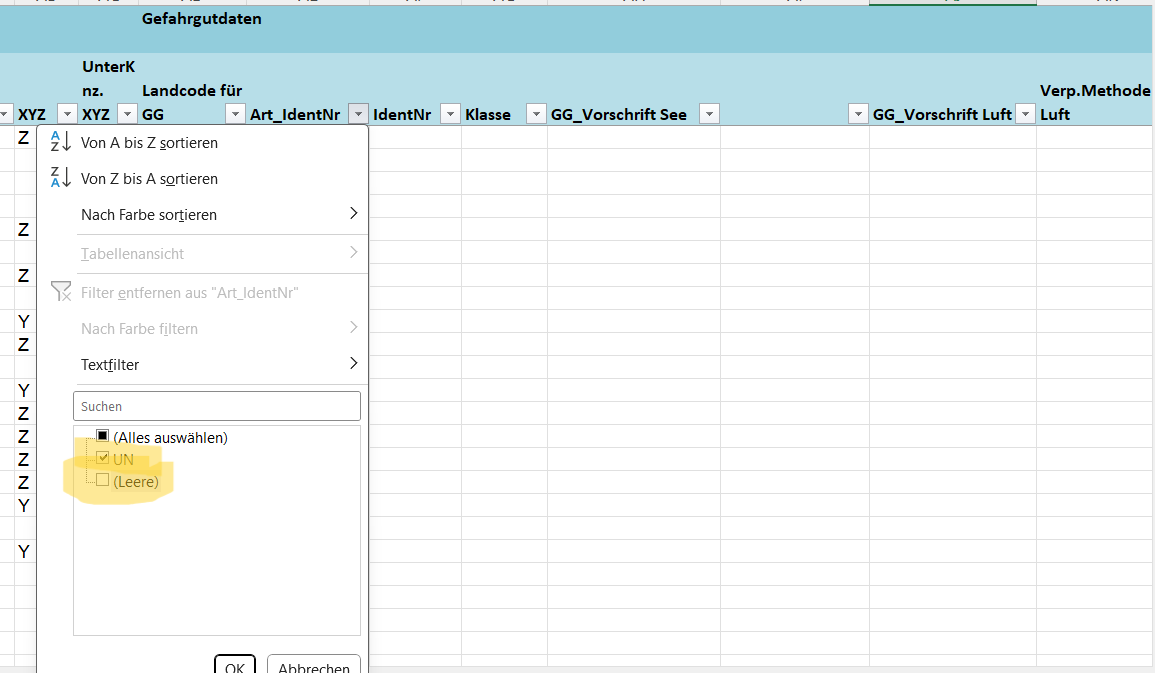
\includegraphics[width=0.7\linewidth]{./assets/gg-filter-art_IdentNr.png}
  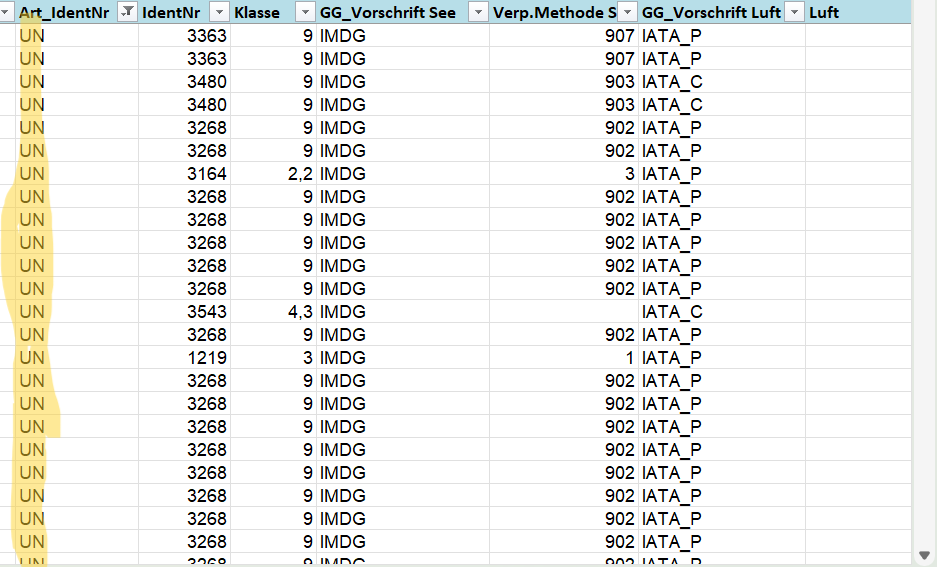
\includegraphics[width=0.7\linewidth]{./assets/gg-un-gefahrgut.png}
\end{center}


\subsection{Fokus auf Lufttransport-Vorschriften}
Da sich mein Fokus zunächst auf Verpackungsvorschriften für Lufttransporte richtete, wurden besonders die 
Spalten \texttt{GG\_Vorschrift Luft} und \texttt{Verp. Methode Luft} analysiert. Die Filterung der 
\texttt{GG\_Vorschrift Luft} war einfach, da lediglich zwei Varianten vorkamen: IATA\_C und IATA\_P.

\begin{center}
  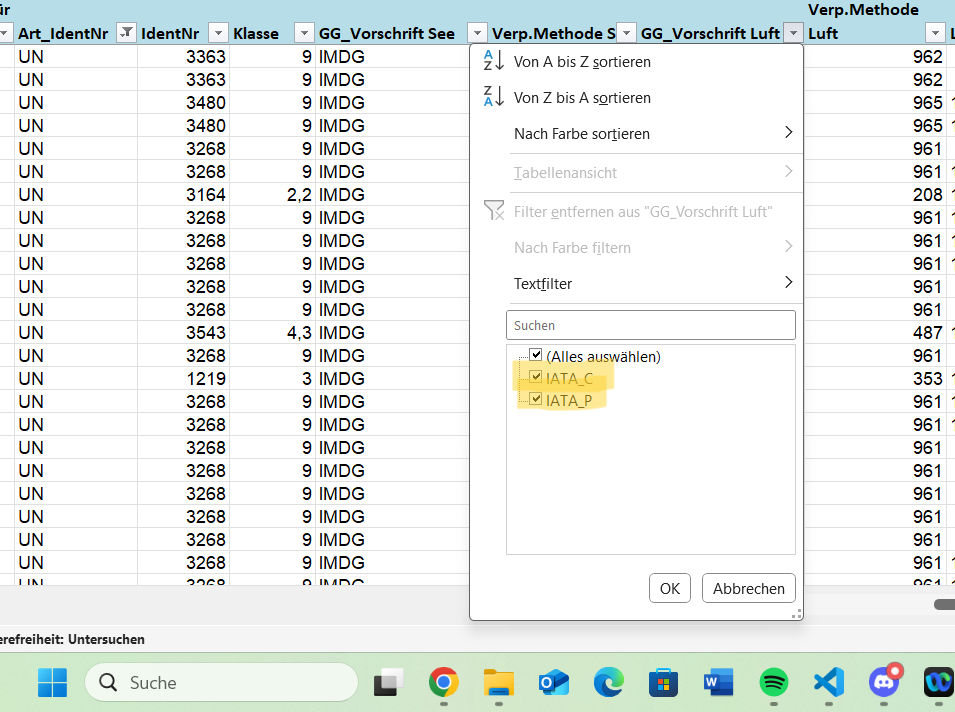
\includegraphics[width=0.7\linewidth]{./assets/gg-GG_vorschrift luft-filter.png}
  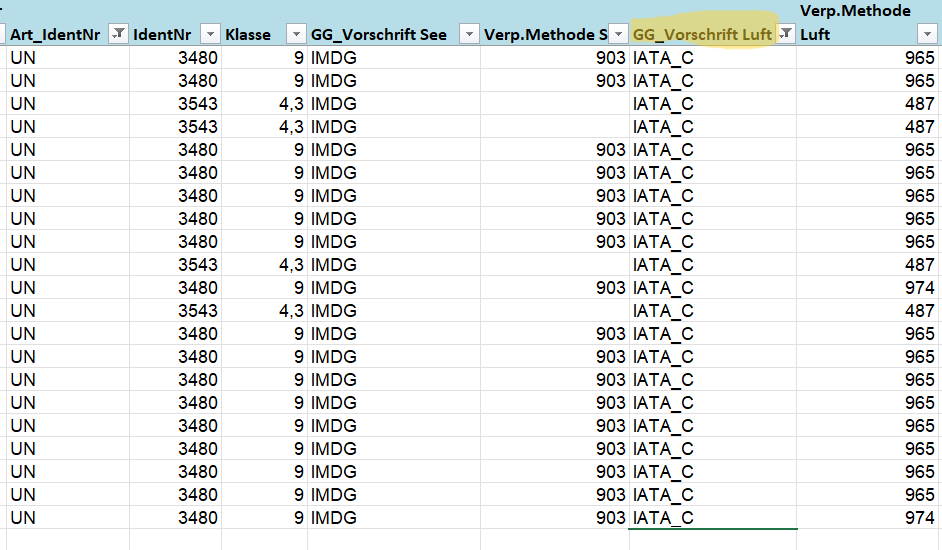
\includegraphics[width=0.7\linewidth]{./assets/gg-GG_vorschrift_luft.png}
\end{center}


Herausfordernder war hingegen die Vielzahl an unterschiedlichen Verpackungsmethoden, die separat gefiltert und 
analysiert werden mussten.

\begin{center}
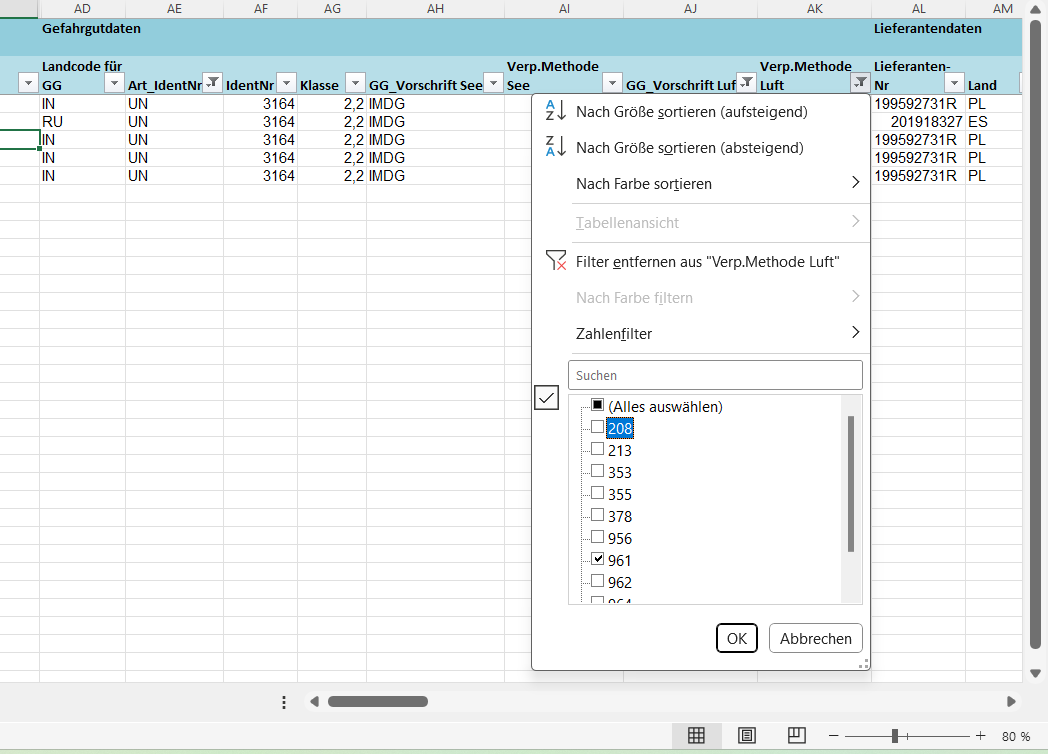
\includegraphics[width=0.7\linewidth]{.assets/gg-verpackungsmethode-filter.png} \\
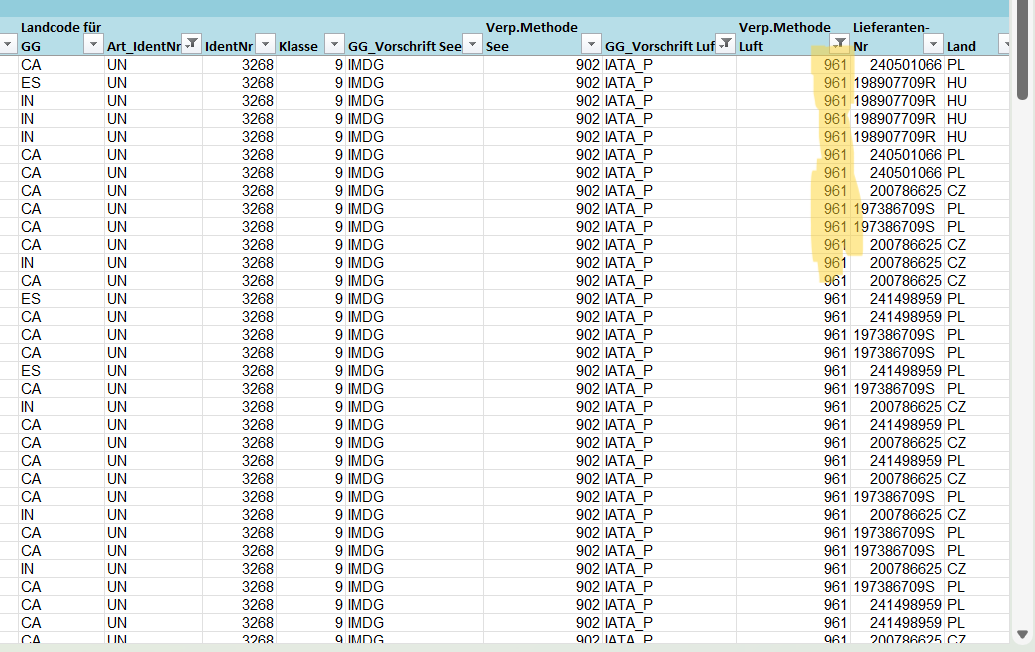
\includegraphics[width=0.7\linewidth]{.assets/gg-verpackungsmethode-nr.png}
\end{center}

\subsection{Abgleich mit Materialien und Modulgruppen}
Ein wichtiger Teil bestand darin, die Gefahrgutinformationen mit den tatsächlichen Materialien und Modulgruppen zu
verknüpfen. Diese standen allerdings in weit entfernten Spalten, in die man erst rüberscrollen musste und so eine 
effiziente Arbeit erschwerte. Um effizienter zu arbeiten, wurden irrelevante Spalten kurzerhand ausgeblendet, um nur 
die für Gefahrgut relevanten Felder gegenüberzustellen.

\begin{center}
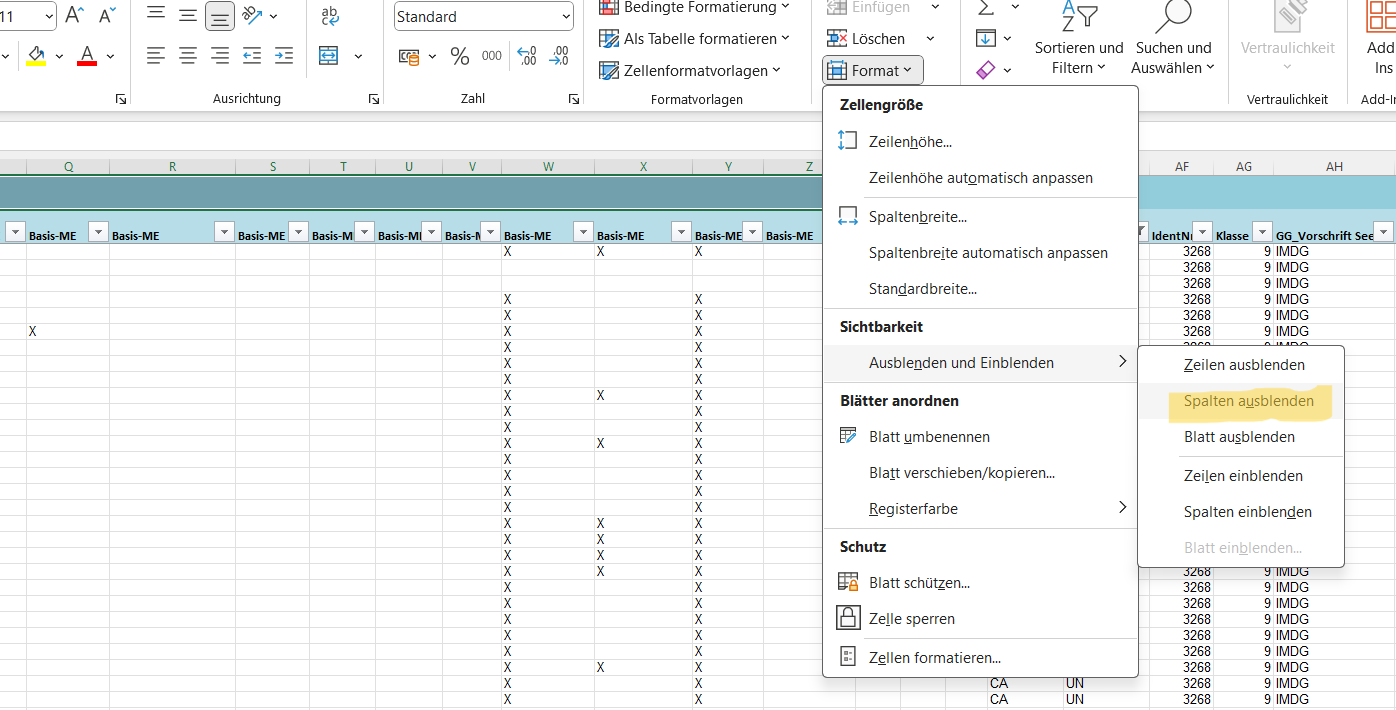
\includegraphics[width=0.85\linewidth]{.assets/gg-unrelevante spalten ausblenden .png} \\
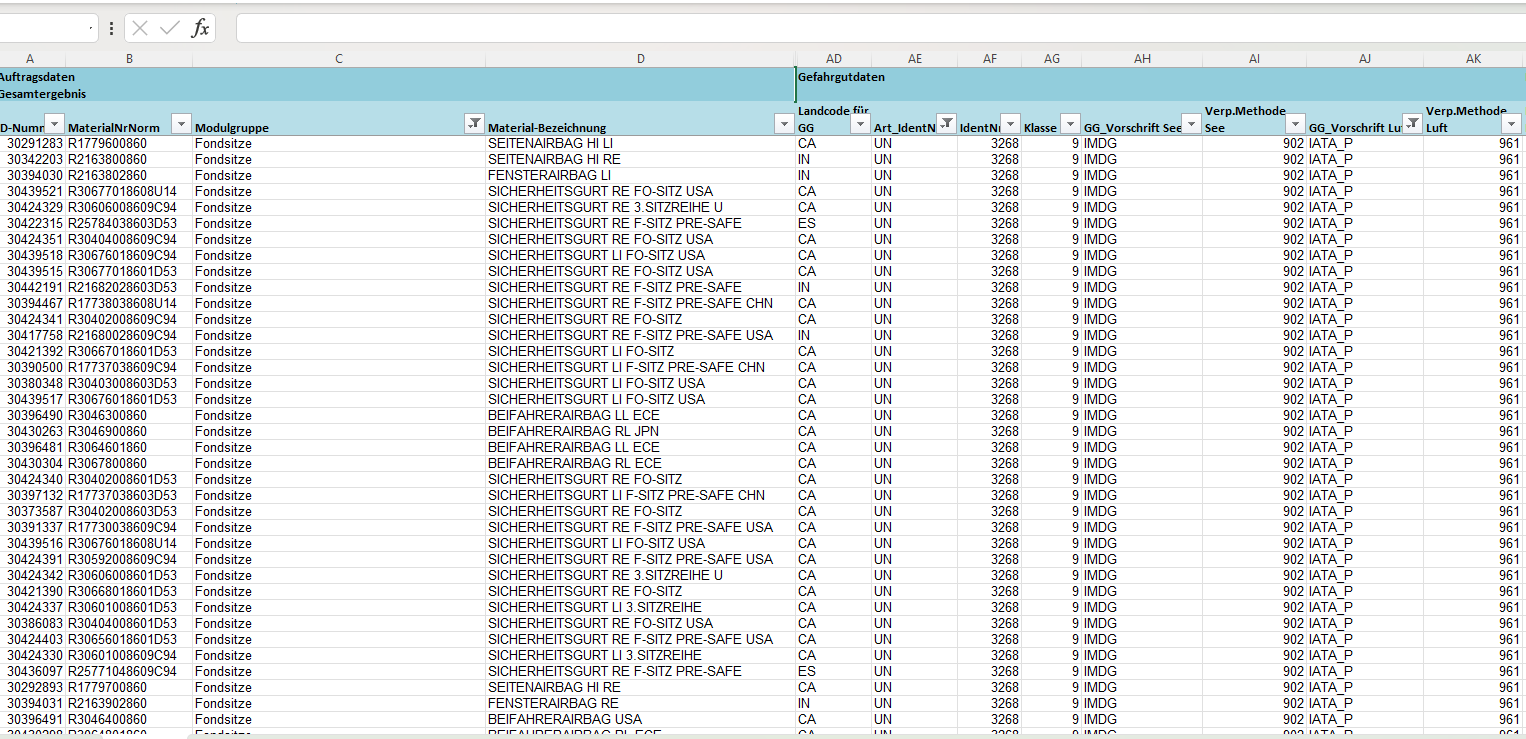
\includegraphics[width=0.85\linewidth]{.assets/gg-gefahrgutrelevante Daten.png}
\end{center}

\subsection{Grenzen und manuelle Entscheidungen}
Sollten Materialien oder Modulgruppen mehrfach vorkommen – in einem Fall als Gefahrgut, im anderen nicht – wurde dies 
im Sinne der Zeitersparnis bewusst vernachlässigt. Die Analyse erfolgte ausschließlich auf Basis der bereitgestellten, 
vorgefüllten Daten.

\subsection{Fazit}
Auch wenn Filter- und Automatisierungsfunktionen in Excel eine erhebliche Erleichterung darstellen, war die manuelle 
Vorarbeit essenziell. Nur durch ein schrittweises, systematisches Herausfiltern konnten die für das Projekt relevanten 
Gefahrgüter und ihre Eigenschaften korrekt isoliert und bearbeitet werden.
